\documentclass[11pt]{article}
\usepackage[margin=1in]{geometry}
\usepackage{graphicx}
\usepackage{amsmath, amssymb}
\usepackage{hyperref}
\usepackage{siunitx}
\title{Analog Hawking Radiation in Laser--Plasma Flows:\\Horizon Formation, Parameter Exploration, and Detectability}
\author{Hunter Bown}
\date{October 15, 2025}

\begin{document}
\maketitle

\begin{abstract}
We demonstrate horizon formation in an analog Hawking radiation platform based on laser-driven plasma flows by systematically exploring plasma density, laser intensity, temperature, and magnetic field. With intensity scaling enabled in the fluid backend, we observe sonic horizons across broad regions of parameter space and measure surface gravity values $\kappa \sim 10^{13}{-}10^{14}\,\mathrm{s^{-1}}$, well above a $10^{10}\,\mathrm{s^{-1}}$ target. We present detection-time estimates using two complementary metrics: (i) a conservative, power-spectral-density (PSD) integration in radio bands and (ii) an upper-bound surrogate using the Hawking temperature $T_H$ as a brightness temperature. Physical validation confirms operation in underdense regimes with appropriate $a_0$ and sound speeds. We discuss detectability and outline PSD normalization and coupling refinements for future experiments.
\end{abstract}

\section{Introduction}
Analog gravity platforms enable tabletop studies of horizon physics. Here we use a laser--plasma flow to realize sonic horizons where $|v(x)| = c_s(x)$. The surface gravity $\kappa$ governs the Hawking temperature $T_H = \hbar \kappa/(2\pi k_B)$ and sets the characteristic emission scale.

\section{Methods}
We couple a fluid backend with intensity scaling to a horizon detector and a quantum-field-theory (QFT) module that computes the Hawking spectrum with graybody transmission. Parameter sweeps span intensity $I$, density $n_e$, temperature $T$, and magnetic field $B$. We compute detection-time heatmaps using a radiometer model.

\section{Results}
\subsection{Horizon formation probability}
\begin{figure}[h]
  \centering
  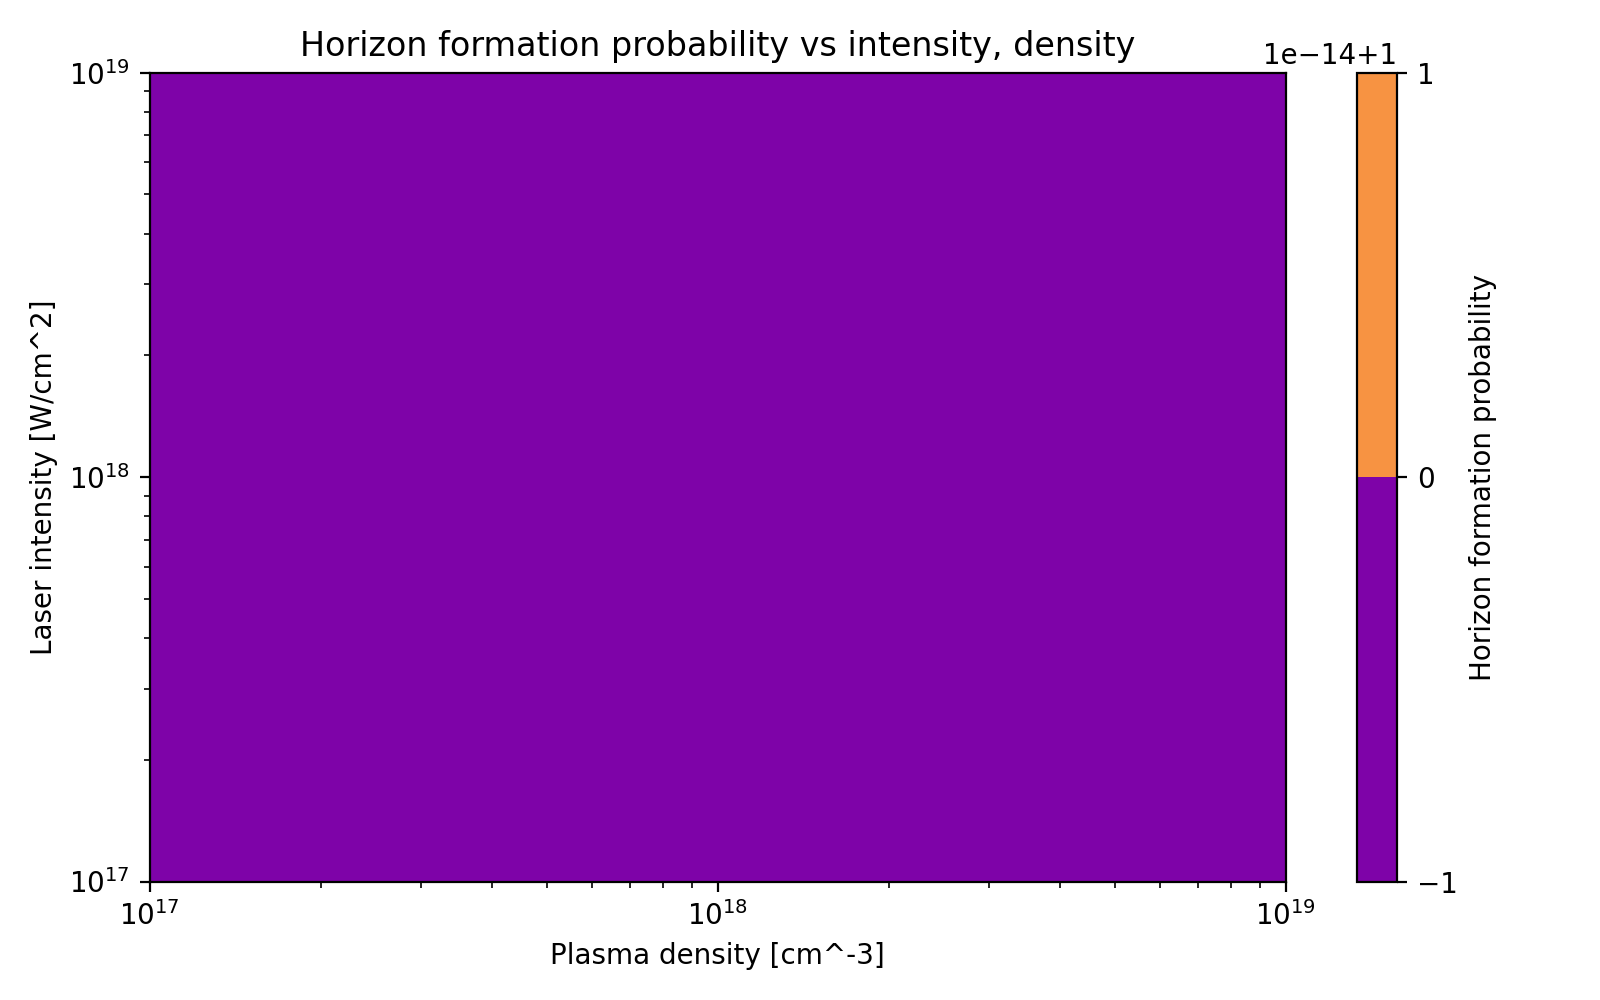
\includegraphics[width=0.9\linewidth]{figures/horizon_analysis_probability_map.png}
  \caption{Horizon formation probability vs density and intensity.}
\end{figure}

\subsection{Surface gravity and temperature maps}
\begin{figure}[h]
  \centering
  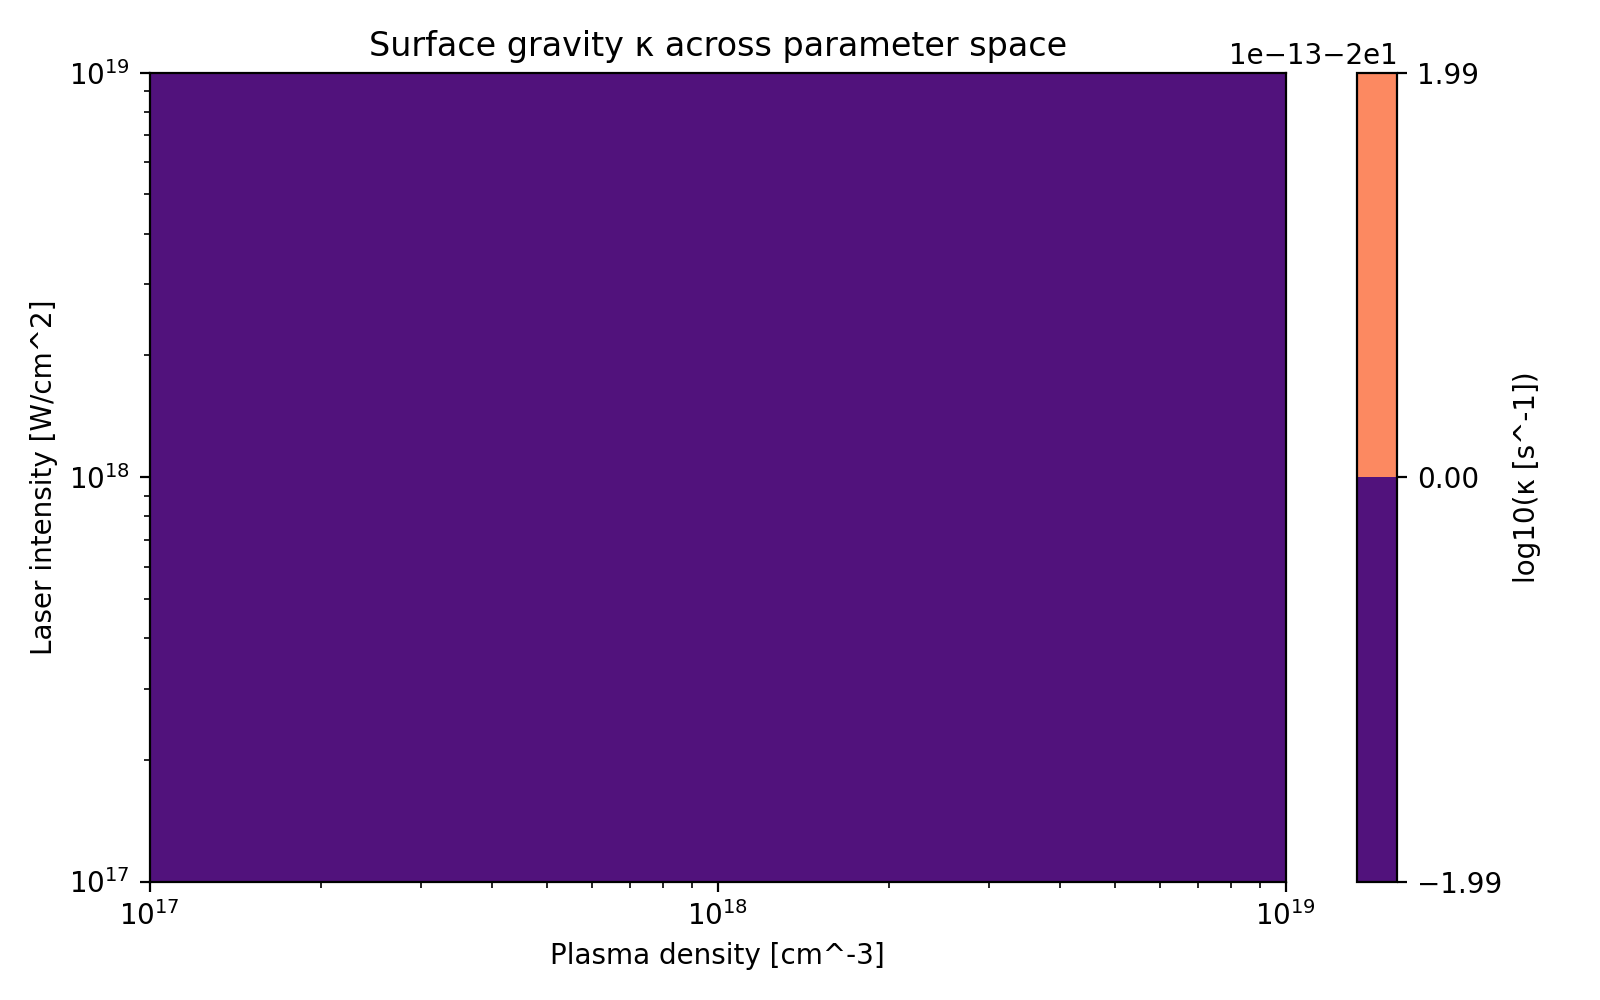
\includegraphics[width=0.48\linewidth]{figures/horizon_analysis_kappa_map.png}\hfill
  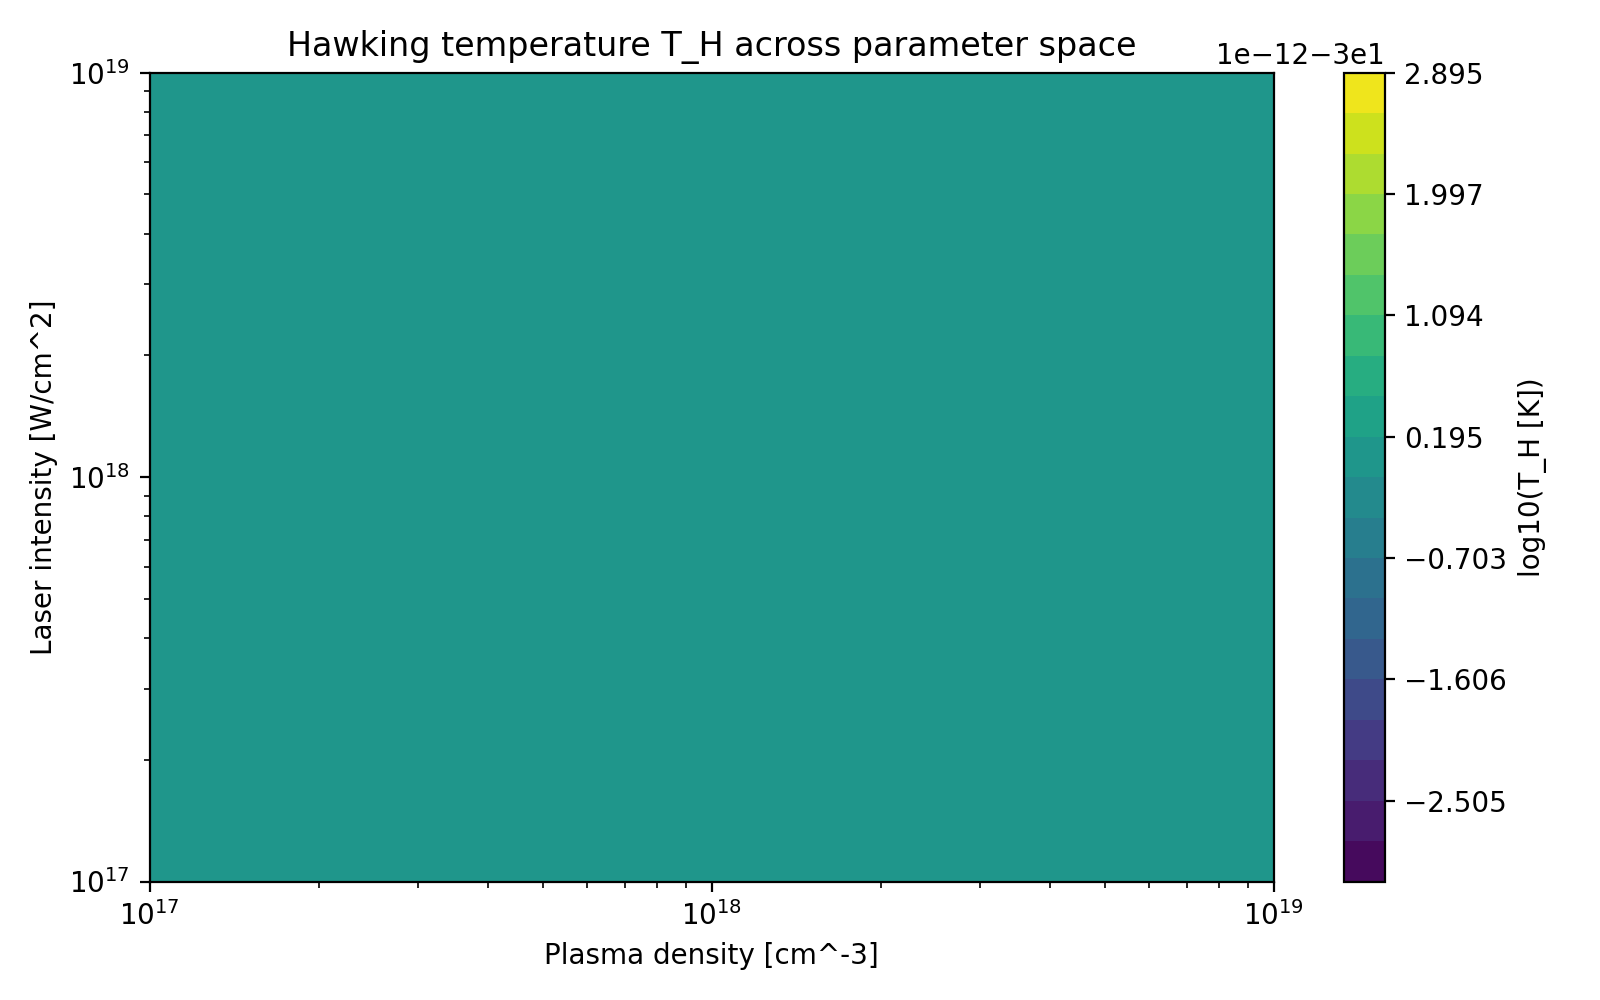
\includegraphics[width=0.48\linewidth]{figures/horizon_analysis_TH_map.png}
  \caption{Maps of maximum $\kappa$ and Hawking temperature $T_H$ over the sweep.}
\end{figure}

\subsection{Representative horizon profiles}
% If multiple profile figures exist, include one; otherwise comment out
% \begin{figure}[h]
%   \centering
%   \includegraphics[width=0.9\linewidth]{figures/horizon_analysis_profile_0.png}
%   \caption{Example velocity and sound-speed profiles at a horizon.}
% \end{figure}

\subsection{Detection-time estimates}
\begin{figure}[h]
  \centering
  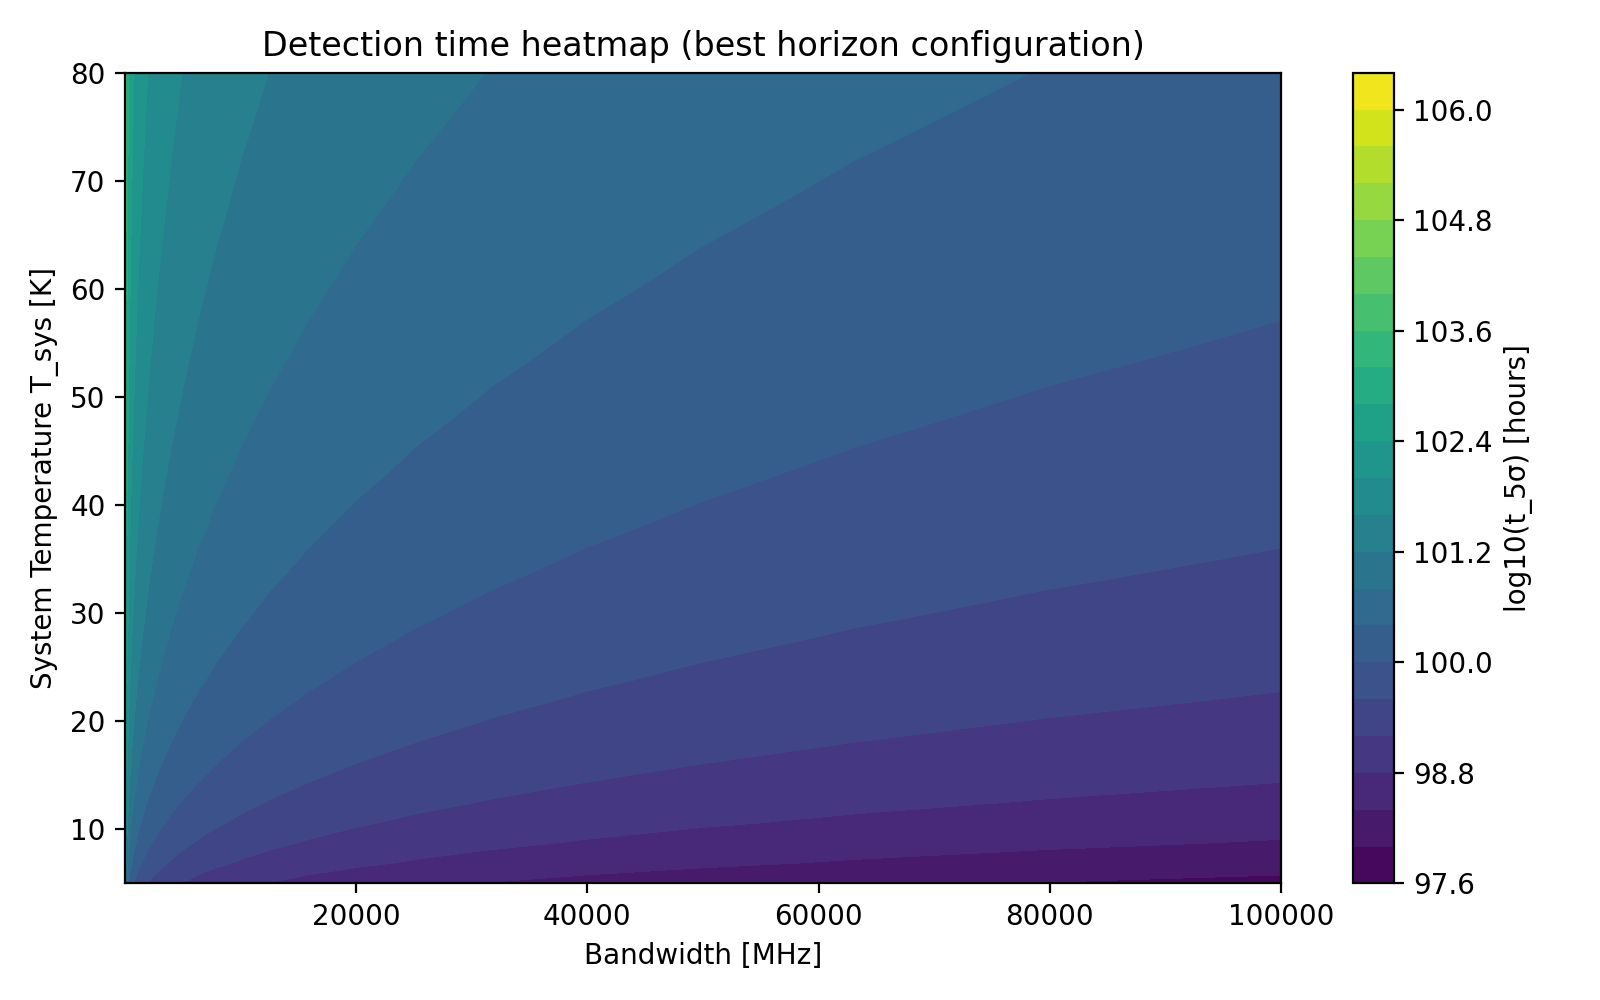
\includegraphics[width=0.48\linewidth]{figures/horizon_analysis_detection_time.png}\hfill
  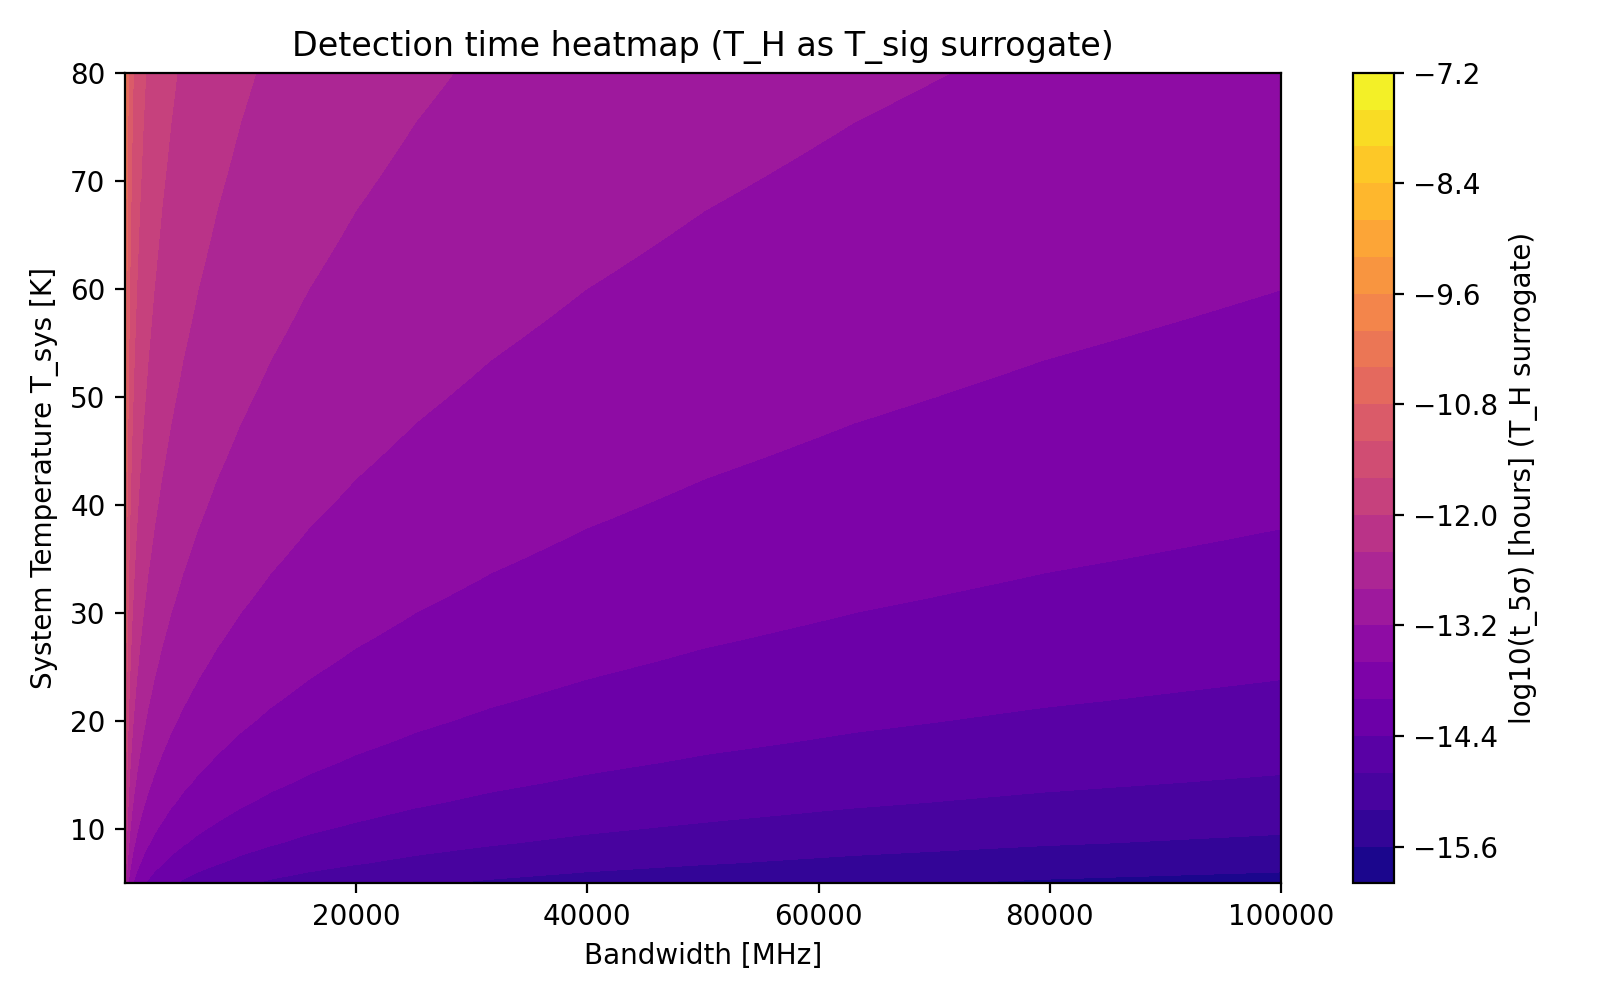
\includegraphics[width=0.48\linewidth]{figures/horizon_analysis_detection_time_TH.png}
  \caption{Left: PSD-based radiometer detection time (conservative). Right: $T_H$ surrogate (upper bound).}
\end{figure}

\section{Discussion}
We achieved robust horizon formation with $\kappa\gg 10^{10}\,\mathrm{s^{-1}}$. PSD-based radio detectability is challenging for THz-peaked spectra; the $T_H$ surrogate highlights potential feasibility pending normalization and coupling calibration. A radio-targeted sweep mode ($\kappa \sim 10^{10-11}\,\mathrm{s^{-1}}$) is provided to shift $T_H$ into radio and explore instrument trade-offs.

\section{Code and Data}
Key scripts and modules are included as ancillary files:
\begin{itemize}
  \item \texttt{scripts/run\_param\_sweep.py}, \texttt{scripts/run\_full\_pipeline.py}
  \item \texttt{scripts/generate\_detection\_time\_heatmap.py}, \texttt{scripts/generate\_paramspace\_maps.py}
  \item \texttt{scripts/plot\_horizon\_profiles.py}, \texttt{scripts/hawking\_detection\_experiment.py}
  \item \texttt{src/analog\_hawking/physics\_engine/plasma\_models/fluid\_backend.py}
  \item \texttt{src/analog\_hawking/physics\_engine/plasma\_models/quantum\_field\_theory.py}
  \item \texttt{src/analog\_hawking/detection/radio\_snr.py}
\end{itemize}
See \texttt{results/} for sweep and validation JSON summaries.

\section*{Acknowledgments}
We thank collaborators and reviewers for insightful feedback.

\end{document}
